%----------------------------------------------------------------------------------------
% Proposta di progetto
%----------------------------------------------------------------------------------------

\documentclass[10pt]{softeng} % Document font size and equations flushed left

%----------------------------------------------------------------------------------------
%	DOCUMENT INFORMATION
%----------------------------------------------------------------------------------------

\Phase{Inception - I iterazione}

\DocumentTitle{Requisiti di progetto} % Document title

%----------------------------------------------------------------------------------------

\begin{document}

\startofdocument{}

\section{Glossario}
%(versione 1 : sono omesse definizioni banali e/o implicite)

\paragraph{Accoppiamento}
\`e il grado di dipendenza di una componente del sistema software dalle altre componenti.
L'accoppiamento \`e un fenomeno negativo in contrapposizione con la coesione.
Alto accoppiamento rende difficile la manutenzione e la modifica del codice.

\paragraph{Audit di sicurezza} 
	operazioni di controllo del sistema effettuate periodicamente per controllare che non ci siano sate violazioni della politica di sicurezza adottata
\paragraph{Banca D'Italia}
	 Banca centrale della Repubblica Italiana, avente funzione sia di vigilanza su banche, istituti di credito, intermediari finanziari sia di principale controllore in materia di antiriciclaggio: insieme alla CONSOB, deve avere libero accesso, entro i termini previsti dalla legge, ai dati contenuti nei database di qualsiasi istituto finanziario che operi sul territorio italiano. \cite{banca_italia}
\paragraph{Bonifico}     
	operazione bancaria mediante la quale si mette a disposizione di una persona o le si accredita una somma di denaro per ordine e conto di altri
\paragraph{Bonifico Sepa}
	bonifico (v.bonifico) accreditabile ad un destinatario ubicato oltre i confini nazionali nell'area SEPA.
\paragraph{Conto Corrente (cc)}
	indica un deposito di danaro effettuato dal possesore del bene, detto \emph{correntista}, in una banca o istituto di credito
\paragraph{Codice IBAN}
	L'International Bank Account Number è uno standard internazionale utilizzato per identificare un'utenza bancaria e/o operazione associata ad un conto corrente 
\paragraph{Codice BIC/SWIFT}
	standard che definisce i \emph{bank identifier codes} (codici d'identificazione bancaria) approvato dall'International Organization for Standardization (ISO). Questi codici vengono utilizzati per i trasferimenti di denaro tra banche, specialmente nelle transazioni internazionali, per le quali è spesso ancora necessario nonostante l'entrata in vigore dell'IBAN. \cite{bic_wiki}
\paragraph{Commissione Nazionale per le societ\`a e la borsa (CONSOB)}
	è un'autorità amministrativa indipendente, dotata di personalità giuridica e piena autonomia la cui attività è rivolta alla tutela degli investitori, all'efficienza, alla trasparenza e allo sviluppo del mercato mobiliare italiano. \cite{consob_wiki}
\paragraph{Downtime}
termine inglese per rappresentare il tempo di fermo di un sistema informatico.
Puo essere dovuto alla manutenzione programmata oppure al malfunzionamento.
Opposto di Uptime.
\paragraph{Fondo comune di investimento}
	è un istituto d'intermediazione finanziaria mediante il quale è possibile partecipare, investita una determinata quota di danaro, alla gestione e alla spartizione di dividendi prodotti da un determinato \emph{bene mobiliare} nel tempo. La \emph{banca depositaria} ne custodisce materialmente i titoli e ne tiene in cassa le disponibilità liquide. Le banche hanno inoltre un ruolo di controllo sulla legittimità delle attività del fondo sulla base di quanto prescritto dalle norme della Banca d'Italia e dal regolamento del fondo stesso
\paragraph{Istituto di credito}
	organismo che svolge simultaneamente l’attività di raccolta di risorse finanziarie e di concessione del credito per proprio contoa terzi 
\paragraph{Microservizio}
unit\`a software indipendente progettata per svolgere un singolo compito specifico. Insieme pi\`u microservizi formano un sistema modulare a basso accoppiamento. In un sistema orientato a microservizi un modulo \`e facilmente rimpiazzabile senza compromettere la funzionalit\`a del sistema.

\paragraph{Open Bank Project (OBP)}
	è una API open source che permette a banche ed istituti di credito di creare un interfaccia utente di ampia portata e fruibilità. Essendo un sistema molto versatile e largamente riadattabile, si presta molto a definire un vero e proprio \emph{standard di interfaccia}, ossia a definire un canone per la creazione di interfacce rivolte e all'utenza bancaria generica e agli organismi deputati al controllo bancario. \cite{obp}
\paragraph{Portafoglio valori/titoli azionari}
	è l'insieme dei diversi titoli finanziari e/o fondi d'investimento che l'utente bancario generico può possedere.Ogni titolo e/o fondo acquisito viene inserito nel portafoglio.
\paragraph{Refactoring}
	processo di riutilizzazzione di codice già scritto in precedenza, senza doverne generare di nuovo
\paragraph{SEPA}
	La SEPA (Single Euro Payments Area) è l’area unica in cui i cittadini, le imprese e gli enti, possono eseguire e ricevere pagamenti in Euro, all’interno dei confini nazionali e tra i paesi diversi che compongono l’area SEPA con condizioni di base, diritti ed obblighi uniformi tra i paesi stessi. 
\paragraph{Time-based One Time Password (TOTP)}
	è un algoritmo che calcola una \emph{One-Time password} combinando mediante una funzione hash una chiave segreta condivisa ed il tempo corrente. \cite{totprfc}
\paragraph{TLS - Transport Layer Security}
Un protocollo di comunicazione sicura. Usa gli algoritmi di crittografia per garantire una comunicazione sicura fra due terminali informatici su una rete che usa il protocollo tcp/ip.
Garantisce inoltre l'autenticit\`a e l'integrit\`a dei messaggi trasmessi.
Conosciuto anche come SSL.
\paragraph{Trading online}
	pratica uguale a quella del \emph{trading} bancario classico mediante aiuto di personalità con competenze specifiche(v.broker), effettuata però in rete, disponendo cioè di opportuni strumenti software per il monitoraggio di mercati azionari nazionali e internazionali e  per il controllo completo e \emph{real time} del proprio portafoglio azionario.
\paragraph{Uptime}
    termine inglese che denota il tempo in cui il sistema informatico \`e attivo e funziona correttamente.
    Opposto di Downtime.


\paragraph{VPN - Virtual Private Network}
        \`e una tecnologia per estendere una rete informatica privata, sfruttando come strato sottostante una rete publica.
    Definisce una serie di protocolli di comunicazione e crittografia che permettono la comunicazione sicura ed affidabile.
    Una VPN permette di avere gli stessi vantaggi di una linea privata, ma a un costo significativamente inferiore.
\subsection{Virtualizzazione}
\paragraph{Virtualizzazione dell'hardware}
\`e una tecnologia dove il sistema operativo non viene eseguito direttamente su una macchina fisica, ma viene creata una macchina virtuale che emula il comportamento della macchina fisica. In genere il sistema operativo e i processi che girano sulla macchina virtuale non sono influenzati dai processi esterni alla macchina virtuale, ma possono comunicare.
Usando questo approccio le componenti hardware vengono emulate in software, introducendo overhead.
Questo approccio offre molti vantaggi come flessibilit\`a e indipendenza dalla piattaforma.
\paragraph{Virtualizzazione al livello del sistema operativo}
\`e una tecnologia dove il kernel del sistema operativo viene eseguito sulla macchina fisica. Il software di virtualizzazione \`e una parte del kernel. I processi vengono eseguiti all'interno dei container, che sono isolati fra loro, e non possono interferire con i processi negli altri container. I container tuttavia possono essere configurati per permettere la comunicazione.
Ogni processo viene esegito direttamente sulla CPU fisica della macchina, e l'hardware non viene emulato.
In genere la virtualizzazione al livello del sistema operativo ha performance migliori rispetto alla virtualizzazione hardware.



\section{Ripulire...}


Un utente registrato pu\`o ottenere una lista delle tipologie di servizi offerti dalla banca che pu\`o sottoscrivere.

Un utente pu\`o aprire diversi tipi di conto corrente, 

Un utente titolare di un conto.

Audit di sicurezza:
storico delle connessioni e delle operazioni riguardanti il conto corrente.

Il sistema di home banking \`e personalizzabile dagli impiegati della banca.
I dipendenti della banca possono creare:
- conti di deposito
- carte di credito/debito
Personalizzando vari parametri.
I dirigenti possono permettere l'apertura di certi conti/carte solo a clienti che abbiano i requisiti specificati:
- giacenza media
- capitale depositato che aumenta
- boh

Possibilit\`a di bidding in cui un utente fa una proposta alla banca per ottenere un conto o una carta con certe particolari condizioni/agevolazioni.
In base a delle regole definite dai dirigenti questa proposta pu\`o essere:
- approvata automaticamente dal sistema
- inoltrata a un manager per l'approvazione
- rifiutata automaticamente
Controllare se la cosa \`e legale o se ce ne freghiamo.



%--------------------------------------------------------------

% TODO ripulire questa parte e spostare tutto nel file dei requisiti
Per rafforzare i requisiti non funzionali (come i requisiti di sicurezza) si sceglie di rivolgere il sistema di Home Banking a persone fisiche (retail banking).

Alcune delle funzionalit\`a che il sistema pu\`o offrire sono:
\begin{enumerate}
	\item L'utente si deve poter pre-registrare online fornendo i suoi dati anagrafici, e:
		\begin{enumerate}
			\item se l'utente ha gi\`a un conto aperto con la banca, pu\`o fornire il suo numero di conto;
			\item se l'utente non ha gi\`a un conto con la banca, pu\`o scegliere diverse soluzioni con agevolazioni differenti e pre-compilare i moduli necessari all'apertura del conto.
				% TODO: cambiare "se l'utente ha gi\`a un conto con la banca" in "se l'utente desidera aprire un nuovo conto"
		\end{enumerate}
		Un utente pre-registrato pu\`o recarsi presso una filiale della banca e ultimare la registrazione presentando il documento d'identit\`a.
		La banca gli fornir\`a le informazioni per l'accesso.
		Ai nuovi clienti viene fornito su richiesta un bancomat.
		% TODO: rimuovere, non \`e di interesse per l'applicazione, facciamo home banking non ATM

		Un utente non pre-registrato pu\`o effettuare la procedura completa di registrazione presso una filiale, fornendo le stesse informazioni richieste agli utenti che si pre-registrano online.
	\item Le informazioni per l'accesso comprendono:
		\begin{enumerate}
			\item Il numero di conto;
			\item La password del conto;
			\item Un dispositivo TOTP\footnote{Time-Based One Time Password, RFC 6238. \url{https://tools.ietf.org/html/rfc6238}} per effettuare operazioni sensibili.
		\end{enumerate}
	\item Un utente registrato pu\`o effettuare il login al sistema di Home Banking fornendo le informazioni di accesso (requisito TOT), in particolare deve inserire numero di conto e password del conto.
	\item Un utente che ha effettuato l'accesso al sistema di Home Banking deve poter svolgere le seguenti operazioni senza fornire la One Time Password:
		\begin{enumerate}
			\item Visionare saldo contabile, disponibile e liquido.
			\item Visionare uno storico delle transazioni effettuate.
			\item Visionare informazioni riguardo le carte di credito collegate al conto (se presenti).
			\item Effettuare ``operazioni veloci'' impostate attraverso un sistema di configurazione (requisito TOT).
		\end{enumerate}
	\item Un utente che ha effettuato l'accesso al sistema di Home Banking deve poter effettuare le seguenti operazioni fornendo ogni volta la One Time Password:
		\begin{enumerate}
			\item Effettuare transazioni, come:
				\begin{enumerate}
					\item bonifici ordinari e bonifici SEPA;
					\item ricariche carte prepatate e schede telefoniche;
					\item pagamento bollette, bollettini, tasse, etc;
				\end{enumerate}
			\item Configurare operazioni veloci.
			\item Se ci viene in mente altro ce lo mettiamo.
		\end{enumerate}
	\item Ogni operazione deve essere registrata in un log.
		Devono essere mantenute le seguenti informazioni:
		\begin{enumerate}
			\item l'operazione eseguita;
			\item il conto coinvolto nell'operazione;
				% TODO rivedere codesta parte: codice univoco della transazione al posto del conto?
				% analizzare bene come funziona OBP
			\item l'istante dell'operazione;
			\item informazioni riguardanti il terminale da cui \`e stata effettuata l'operazione.
		\end{enumerate}
	\item Il sistema deve poter essere configurabile dall'utente per inviare notifiche via SMS e/o via email a seguito di ogni evento stabilito dall'utente.
		La banca pu\`o associare una tariffa per abilitare le notifiche su specifici insiemi di eventi.
		Gli eventi notificabili possono includere:
		\begin{enumerate}
			\item Accesso al sistema;
			\item Pagamento o prelievo dal conto;
			\item Pagamento ricevuto.
		\end{enumerate}
\end{enumerate}

%----------------------------------------------------------------------------------------
%	REFERENCE LIST
%----------------------------------------------------------------------------------------

\nocite{banca_italia}
\printcustombib{}

%----------------------------------------------------------------------------------------
%	FIGURES
%----------------------------------------------------------------------------------------

\begin{figure*}[hbt]
	\centering
	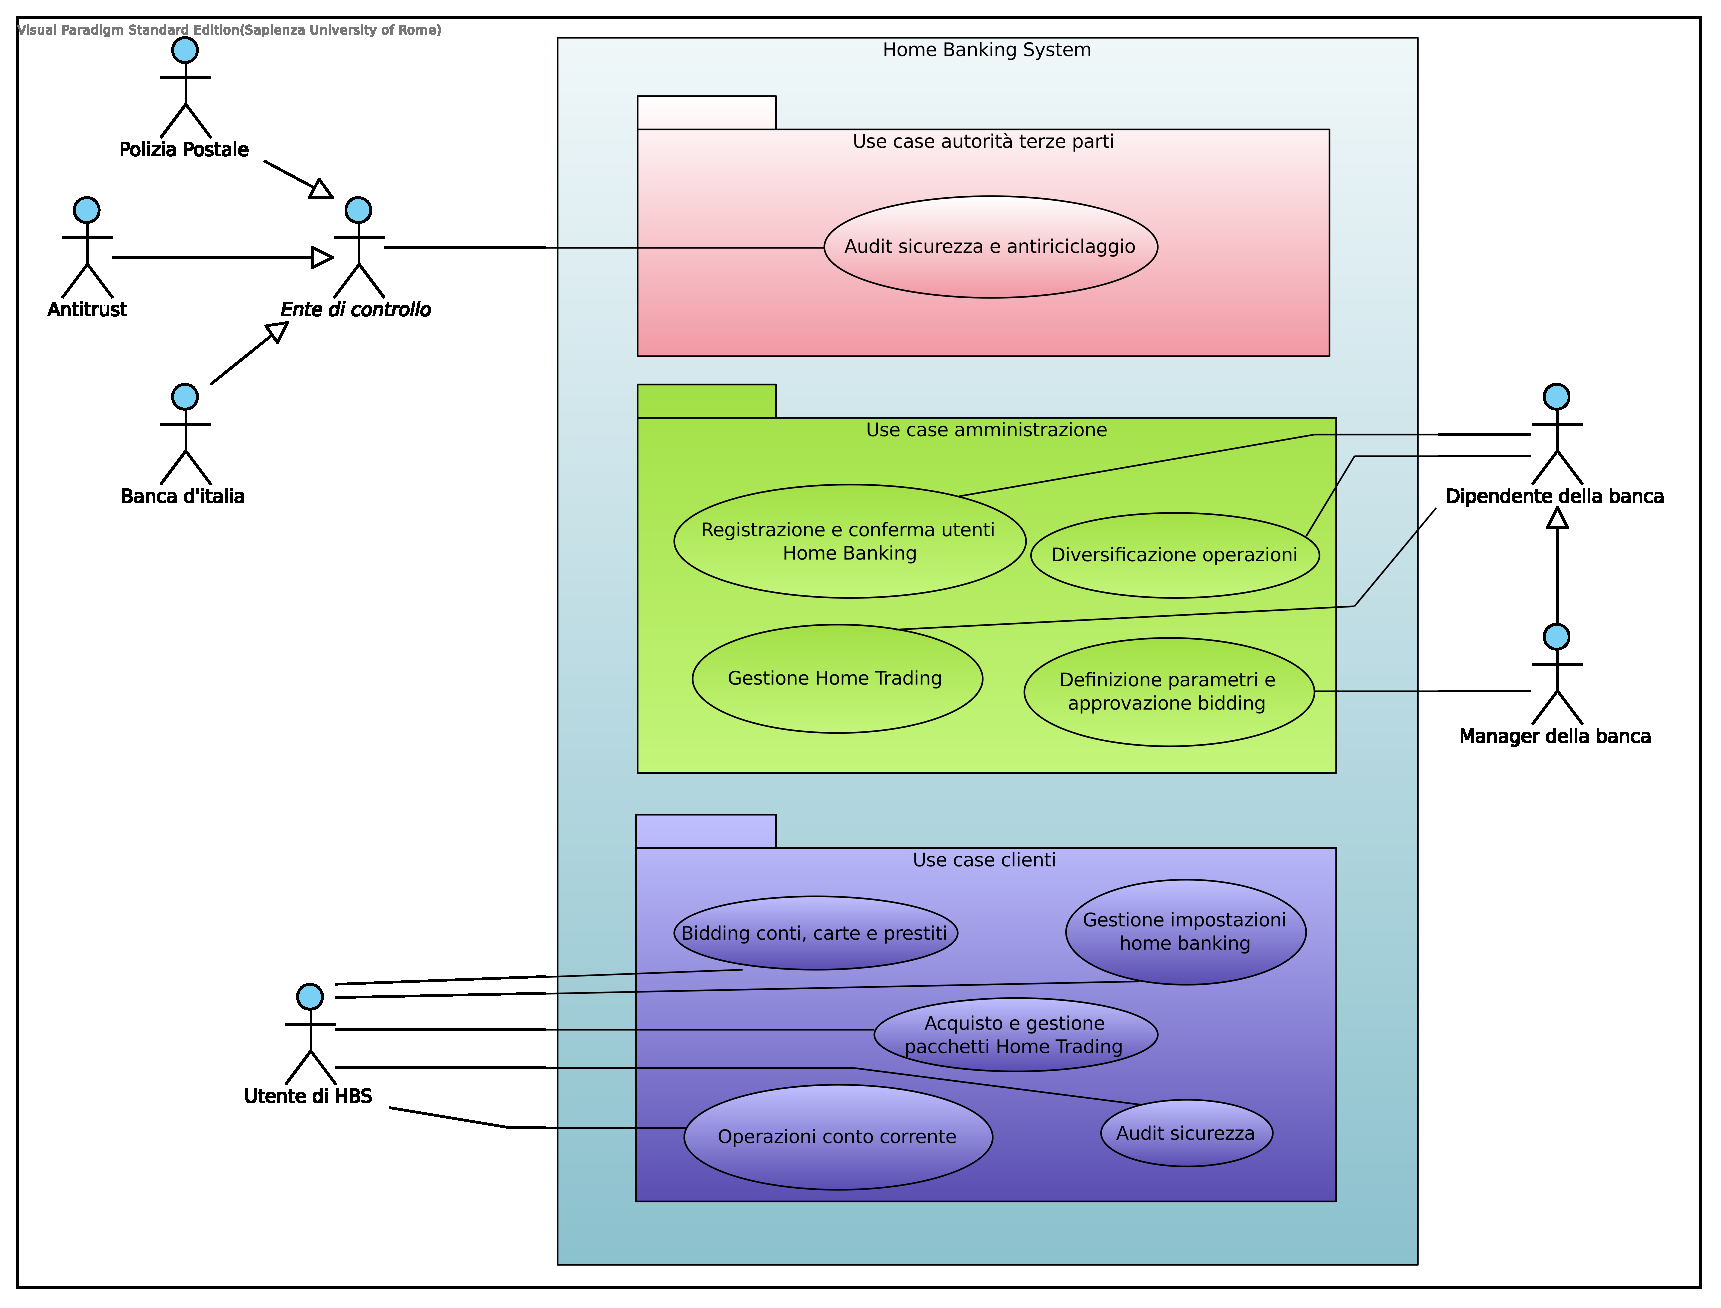
\includegraphics[width=\textwidth]{Images/Home_Banking_inception_use_cases.eps}
	\caption{Attori del sistema di Home Banking e relativi use cases.}
	\label{fig:inception_use_cases}
\end{figure*}

\end{document}
